\documentclass[manuscript,nonacm]{acmart}
\usepackage[T1]{fontenc}
\usepackage{lmodern}

% Turn off ACM copyright footer + author block
\settopmatter{printacmref=false}
\renewcommand\authorsaddresses{}

% Optional: declare no date or set your own
\date{}

% Add packages you need
\usepackage{float}
\usepackage{booktabs}
\usepackage{hyperref}
\usepackage{graphicx}
\usepackage{pdflscape}
\usepackage{amsmath}
\let\Bbbk\relax
\usepackage{amssymb}
\usepackage[utf8]{inputenc}
\usepackage{newunicodechar}
\newunicodechar{∀}{\ensuremath{\forall}}
\newunicodechar{∧}{\ensuremath{\wedge}}

% Optional: for tables with wrapping columns
\usepackage{array}
\newcolumntype{P}[1]{>{\raggedright\arraybackslash}p{#1}}

% Optional: tighter spacing if needed
% \linespread{0.97}

%%
%% \BibTeX command to typeset BibTeX logo in the docs
\AtBeginDocument{%
  \providecommand\BibTeX{{%
    Bib\TeX}}}

%%
%% end of the preamble, start of the body of the document source.
\begin{document}

%%
%% The "title" command has an optional parameter,
%% allowing the author to define a "short title" to be used in page headers.
\title{The Gödel Mirror: Self-Recursive Architectures for Emergent Cognition via Contradiction Resolution}

%%
%% The "author" command and its associated commands are used to define
%% the authors and their affiliations.
%% Of note is the shared affiliation of the first two authors, and the
%% "authornote" and "authornotemark" commands
%% used to denote shared contribution to the research.
\author{Jhet Chan}
\orcid{0009-0008-4363-2979}
\affiliation{%
  \institution{Independent Researcher}
  \city{Kuala Lumpur}
  \country{Malaysia}}
\email{jhetchan@gmail.com}

%%
%% By default, the full list of authors will be used in the page
%% headers. Often, this list is too long, and will overlap
%% other information printed in the page headers. This command allows
%% the author to define a more concise list
%% of authors' names for this purpose.
\renewcommand{\shortauthors}{J. Chan (Gödel Mirror)}

%%
%% The abstract is a short summary of the work to be presented in the
%% article.
\begin{abstract}
  We introduce the \textbf{Gödel Mirror}, a formal cognitive microarchitecture defined in Lean 4 that treats \textbf{contradiction as a control signal} for recursive self-evolution. Inspired by Gödelian self-reference and paraconsistent reasoning, our system encodes symbolic paradoxes as structured transitions between \texttt{MirrorSystem} state. Unlike black-box LLM agents or reward-driven optimizers, the Gödel Mirror is minimal, mechanistically transparent, and \textbf{machine-verifiable}.
\par
  We defined the inductive types, evaluator logic, and agent engine comprising the architecture. Four formal theorems prove that paradoxes are deterministically embodied, recursively re-entered, and transformed into new structures. This yields a \textbf{self-referential inference loop}:

  \texttt{paradox → embody → reenter → node}.
\par
  We argue that this microkernel opens a new class of symbolic systems in which contradiction fuels growth, laying the groundwork for future integrations with perception, language, or reflection-capable agents.
\end{abstract}

%%
%% Keywords. The author(s) should pick words that accurately describe
%% the work being presented. Separate keywords with commas.
\keywords{Gödelian recursion, paradox resolution, emergent cognition, symbolic AI, recursive agents, contradiction-driven inference}

%%
%% This command processes the author and affiliation and title
%% information and builds the first part of the formatted document.
\maketitle

\section{Introduction}
This work draws inspiration from foundational research in formal logic and cognitive modeling, particularly Gödel\cite{godel1931incompleteness}'s treatment of self-reference, the Curry–Howard correspondence\cite{curryhoward} between proofs and programs, and Hofstadter\cite{hofstadter1979geb}'s explorations of recursive systems and symbolic identity. While this paper focuses on formalizing a symbolic framework within a type-theoretic context, a forthcoming companion paper will explore the broader implications of meta-symbolic cognition, embodiment, and recursive meaning-making.

\section{Related Work}
The study of self-reflective agents spans formal logic, recursive self-improvement (RSI), and neuro-symbolic cognition. However, most systems treat contradictions as error states. This paper reframes contradiction as a driver of structured self-growth — a Gödelian feedback loop embedded in type theory\cite{martinlof1984intuitionistic}.

\subsection{Self-reference and Recursive Self-Improvement}
Gödel’s original “self-improving machine” proposal (Schmidhuber, 2003)\cite{schmidhuber2003godel} launched a long lineage of agents that modified their own code. The most recent exemplar is the Gödel Agent (Yin et al., 2025)\cite{yin2025godelagent}, which leverages an LLM scaffold to monkey-patch its Python modules at run-time. Parallel efforts such as STOP (Zelikman et al., 2023)\cite{zelikman2023stop}, the Self-Improving Coding Agent (Robeyns et al., 2025)\cite{robeyns2025sica}, and Looped Transformers for Reasoning (Saunshi et al., 2025)\cite{saunshi2025looped} follow similar patterns, where performance feedback triggers recursive refinements or self-referential inference loops. \footnote{See \autoref{tab:comparison} for a side-by-side comparison of prior self-improvers.}

Other studies, such as Self-Refine (Madaan et al., 2023)\cite{madaan2023selfrefine} operationalize this concept by iteratively critiquing and revising model outputs within a closed LLM loop, showing substantial performance gains in dialogue and reasoning tasks.

Meanwhile, eliminating meta-optimization via self-referential meta-learning (Kirsch \& Schmidhuber, 2022)\cite{kirsch2022selfmeta} proposes a model that learns to optimize its own learning algorithm—a direct instantiation of recursive self-modification within the learning process itself.

While empirically impressive, these systems typically provide no formal guarantees regarding safety, convergence, or transformation logic; recursion remains at the implementation layer. In contrast, the Gödel Mirror formalizes recursion within a typed inductive logic system, offering a machine-verifiable framework for self-reference and symbolic evolution.

\subsection{Reward-centric Autonomy}
A complementary line of research replaces code rewriting with reward shaping. Self-Rewarding Language Models fine-tune themselves by acting as their own evaluators (Yuan et al., 2024)\cite{yuan2024selfrewarding}, and AlphaEvolve explores evolutionary search over agent kernels (DeepMind, 2025)\cite{deepmind2025alphaevolve}. Other frameworks, such as SymbolicAI (Dinu et al., 2024)\cite{dinu2024symbolicai} blend generative models with logic-based modules, where iterative self-evaluation helps refine the reasoning structure over time.

More broadly, the Neuro-Symbolic AI Systematic Review (Colelough et al., 2025)\cite{colelough2025review} reports that while 63\% of surveyed papers address learning and inference, only a small fraction engage with metacognition or contradiction-driven reasoning, highlighting a gap that the Gödel Mirror aims to fill.

These reward-driven or hybrid approaches still treat contradictions as error signals to be minimized rather than as productive computational resources capable of driving symbolic recursion.

\subsection{Paraconsistent Logics and Contradiction Tolerance}
Outside agentic literature, paraconsistent frameworks show that retaining contradictions can be mathematically fruitful. Goertzel (2021)\cite{goertzel2021paraconsistent} maps a four-valued logic onto quantum probability amplitudes, and process-algebra variants permit inconsistent signals without explosion.

More recent work in SymbolicAI (Dinu et al., 2024)\cite{dinu2024symbolicai} demonstrates how logic-based frameworks can support self-referential evaluation and compositional inference graphs, offering a bridge between generative and symbolic reasoning. However, recursion remains modular rather than reflexive.

In parallel, Self-Refine (Madaan et al., 2023)\cite{madaan2023selfrefine} and Looped Models for Reasoning (Saunshi et al., 2025)\cite{saunshi2025looped} adopted iterative feedback loops for LLM refinement, simulating a form of contradiction-driven processing. However, these remain empirical heuristics that are not embedded within a rigorously typed symbolic substrate.

To date, none of these systems have converted contradictions into a deterministic state-transition engine, nor have they offered machine-verified guarantees on recursion safety or emergence semantics.

\subsection{Position of the Gödel Mirror}
The present study bridges these strands. Unlike code-level RSI agents, the \textbf{Gödel Mirror} is defined \textit{inside} type theory: a \texttt{MirrorSystem} structure and a \texttt{MirrorState} evaluator form a Lean-verified machine in which \textbf{contradiction is the control signal}.

Four theorems (see Section 6) prove that every self-referential paradox follows the spiral as follows:

\begin{quote}
paradox → embody → reenter → node
\end{quote}

guaranteeing safety and structural growth.

To the best of our knowledge, this is the first architecture that:

\begin{itemize}
\item (i) formalises contradiction-driven recursion \textit{and}
\item (ii) supplies machine-checked proofs of its invariants.
\end{itemize}
\begin{table}[H]
  \caption{Comparative Summary (selected self-improving agents)}
  \label{tab:comparison}
  \begin{tabular}{@{}llll@{}}
    \toprule
    \textbf{Feature / Model} & \textbf{Gödel Agent (CHAI 2023)} & \textbf{Goertzel's AGI (OpenCog)} & \textbf{This Paper: Gödel Mirror} \\
    \midrule
    \textbf{Recursive Self-Model} & Yes & Yes & Yes (typed inductive loop) \\
    \textbf{Paradox as Engine} & Avoided & Narrative inspiration & Core recursion trigger \\
    \textbf{Formal Proof Backbone} & None & None & Lean 4 proofs \\
    \textbf{Embodied Resolution} & N/A & Simulated embodiment & Structural coherence \\
    \textbf{Symbolic Traceability} & Partial introspection & Unstructured & Deterministic traces \\
    \bottomrule
  \end{tabular}
\end{table}

\paragraph{Key departures from Schmidhuber (2003):}
\begin{tabular}{@{}l l@{}}
\textbf{Paraconsistent logic} $\rightarrow$ &
  contradictions are fuel, not fatal \\[2pt]
\textbf{Continuous micro-reconfiguration} vs.\ &
  one-shot proved rewrites \\[2pt]
\textbf{Emergence metric} $\rightarrow$ &
  replaces scalar utility maximisation
\end{tabular}

This builds on Gödel's insight that any sufficiently expressive system can encode its own meta-structure and echoes Hofstadter's recursive strange loops as generative rather than problematic.

\footnote{A blog post by Filagot (2024) independently discusses mirrors and Gödelian loops in a metaphorical context, but does not introduce a formal model.}

\subsection{Contribution Clarity}
We contribute a \textbf{formal cognitive microarchitecture} in \textbf{Lean 4} where paradoxes are \textbf{recursively embodied} into structure, with \textbf{four mechanistic theorems} establishing its safe evolution, as follows.

\begin{itemize}
\item \textbf{Section 3} defines the theoretical underpinnings of contradiction and embodiment.
\item \textbf{Section 4} formalizes the inductive system and its evaluation rules.
\item \textbf{Section 5} walks through an example trace using Lean code.
\item \textbf{Sections 6–9} develop formal properties, limitations, and future work.
\end{itemize}

This positions the Gödel Mirror as a \textbf{minimal, self-recursive architecture} capable of resolving internal contradictions — a symbolic kernel for emergent cognition.

\section{Conceptual Foundations of the Gödel Mirror}

\subsection{Key Definitions}

\begin{table}[H]
  \caption{Key Concepts of the Gödel Mirror}
  \label{tab:key-concepts}
  \begin{tabular}{@{}ll@{}}
    \toprule
    \textbf{Concept} & \textbf{Definition} \\
    \midrule
    \textbf{Contradiction} & A logical incompatibility between two inferences or states \\
    \textbf{Paradox} & A \textit{stable} contradiction that loops back into itself \\
    \textbf{Node} & A snapshot of the system's current self-representation \\
    \textbf{Reentry} & A recursive return to a prior contradiction, bringing new structure \\
    \textbf{Embodiment} & A resolution not by external validation, but by internal coherence \\
    \textbf{Emergence} & A novel structural insight triggered by traversing contradiction \\
    \bottomrule
  \end{tabular}
\end{table}

\subsection{Gödel Mirror Flow Diagram (Textual)}

\begin{enumerate}
\item \textbf{Contradiction Detected}
\item \textbf{Mirror Step}: Encodes the contradiction as self-reference
\item \textbf{Reentry Loop}: Returns recursively with enriched state
\item \textbf{Embodied Resolution}: Converts contradiction into coherent structure
\item \textbf{Structure Updated}: System grows through paradox spiral
\end{enumerate}

\section{Formal System}

\subsection{Core Types (Lean-style)}

\begin{verbatim}
inductive MirrorSystem : Type
| base : MirrorSystem
| node : MirrorSystem → MirrorSystem
| self_ref : MirrorSystem
| embody : MirrorSystem → MirrorSystem
| reenter : MirrorSystem → MirrorSystem
| named : String → MirrorSystem → MirrorSystem
\end{verbatim}

\subsection{Transition Classifier}

\begin{verbatim}
inductive MirrorState
| Normal 
| Paradox 
| Emergence 
| Reentry
\end{verbatim}

\begin{verbatim}
def classify : MirrorSystem → MirrorState
-- returns state based on pattern-matched structural rules
\end{verbatim}

\subsection{Type Signatures of Evolution}

\begin{itemize}
\item \texttt{step : MirrorAgent → MirrorAgent}\\
    Executes a logic update based on state classification.
    
\item \texttt{embody : MirrorSystem → MirrorSystem}\\
    Triggered by paradox → yields a structural transformation.
    
\item \texttt{reenter : MirrorSystem → MirrorSystem}\\
    Triggered by emergence → yields recursive re-encoding.
\end{itemize}

\subsection{Optional Theoretic Mapping}

\begin{table}[H]
  \caption{Abstract Logic to Gödel Mirror Mapping}
  \label{tab:logic-mapping}
  \begin{tabular}{@{}ll@{}}
    \toprule
    \textbf{Abstract Logic} & \textbf{Gödel Mirror Construct} \\
    \midrule
    Self-reference & \texttt{MirrorSystem.self\_ref} \\
    Meta-level transition & \texttt{embody}, \texttt{reenter} \\
    Fixed point traversal & \texttt{paradox → embody → reenter} \\
    Gödel numbering analog & \texttt{named "Gödel"} or nested names \\
    \bottomrule
  \end{tabular}
\end{table}

\subsection{Well-founded Structure}

Although the Gödel Mirror \textbf{need not terminate}, its transitions are

\begin{itemize}
\item Syntactically meaningful
\item Semantically classifiable
\item Recursively traceable over time
\end{itemize}

This allows reasoning about paradoxes as \textbf{productive}, not blocking.

\begin{quote}
"We now examine what this formal structure guarantees about system behavior."
\end{quote}

\section{Example Run}

This example illustrates the core symbolic recursion loop of the Gödel Mirror in action, using the minimal starting term:

\subsection{Lean Input}

\begin{verbatim}
def custom_start := named "Gödel" (node self_ref)
\end{verbatim}

This seeds the agent with a recursive self-reference labeled \texttt{"Gödel"} triggering an initial paradox.

\subsection{Execution Trace}

\begin{verbatim}
#eval numbered_trace (run_trace custom_start 4)
\end{verbatim}

\textbf{Output:}

\begin{verbatim}
Step 0: Gödel
Step 1: embody
Step 2: reenter
Step 3: node
Step 4: node
\end{verbatim}

\subsection{Step-by-Step Interpretation}

\begin{table}[H]
  \caption{Execution Trace Interpretation}
  \label{tab:execution-trace}
  \begin{tabular}{@{}cllp{7cm}@{}}
    \toprule
    \textbf{Step} & \textbf{Internal Symbol} & \textbf{MirrorState} & \textbf{Lean-to-English Meaning} \\
    \midrule
    0 & \texttt{named "Gödel" (...)} & Paradox & A self-referential symbolic expression was detected. The system flagged this as a paradox. \\
    1 & \texttt{embody(...)} & Emergence & The paradox is internalized — the system enters an insight phase by embodying the contradiction. \\
    2 & \texttt{reenter(...)} & Normal & The insight is reintroduced into the recursive system, allowing normal processing to resume. \\
    3 & \texttt{node(...)} & Normal & Growth continues structurally; no new contradiction is detected. \\
    4 & \texttt{node(...)} & Normal & Recursive expansion proceeds — stable symbolic scaffolding accumulates. \\
    \bottomrule
  \end{tabular}
\end{table}

This sequence demonstrates a full paradox cycle: \textbf{contradiction → embodiment → re-entry → recursive growth}.

\subsection{Visual Trace}

\textbf{A "Mirror Loop" State Machine}

\begin{figure}[H]
    \centering
    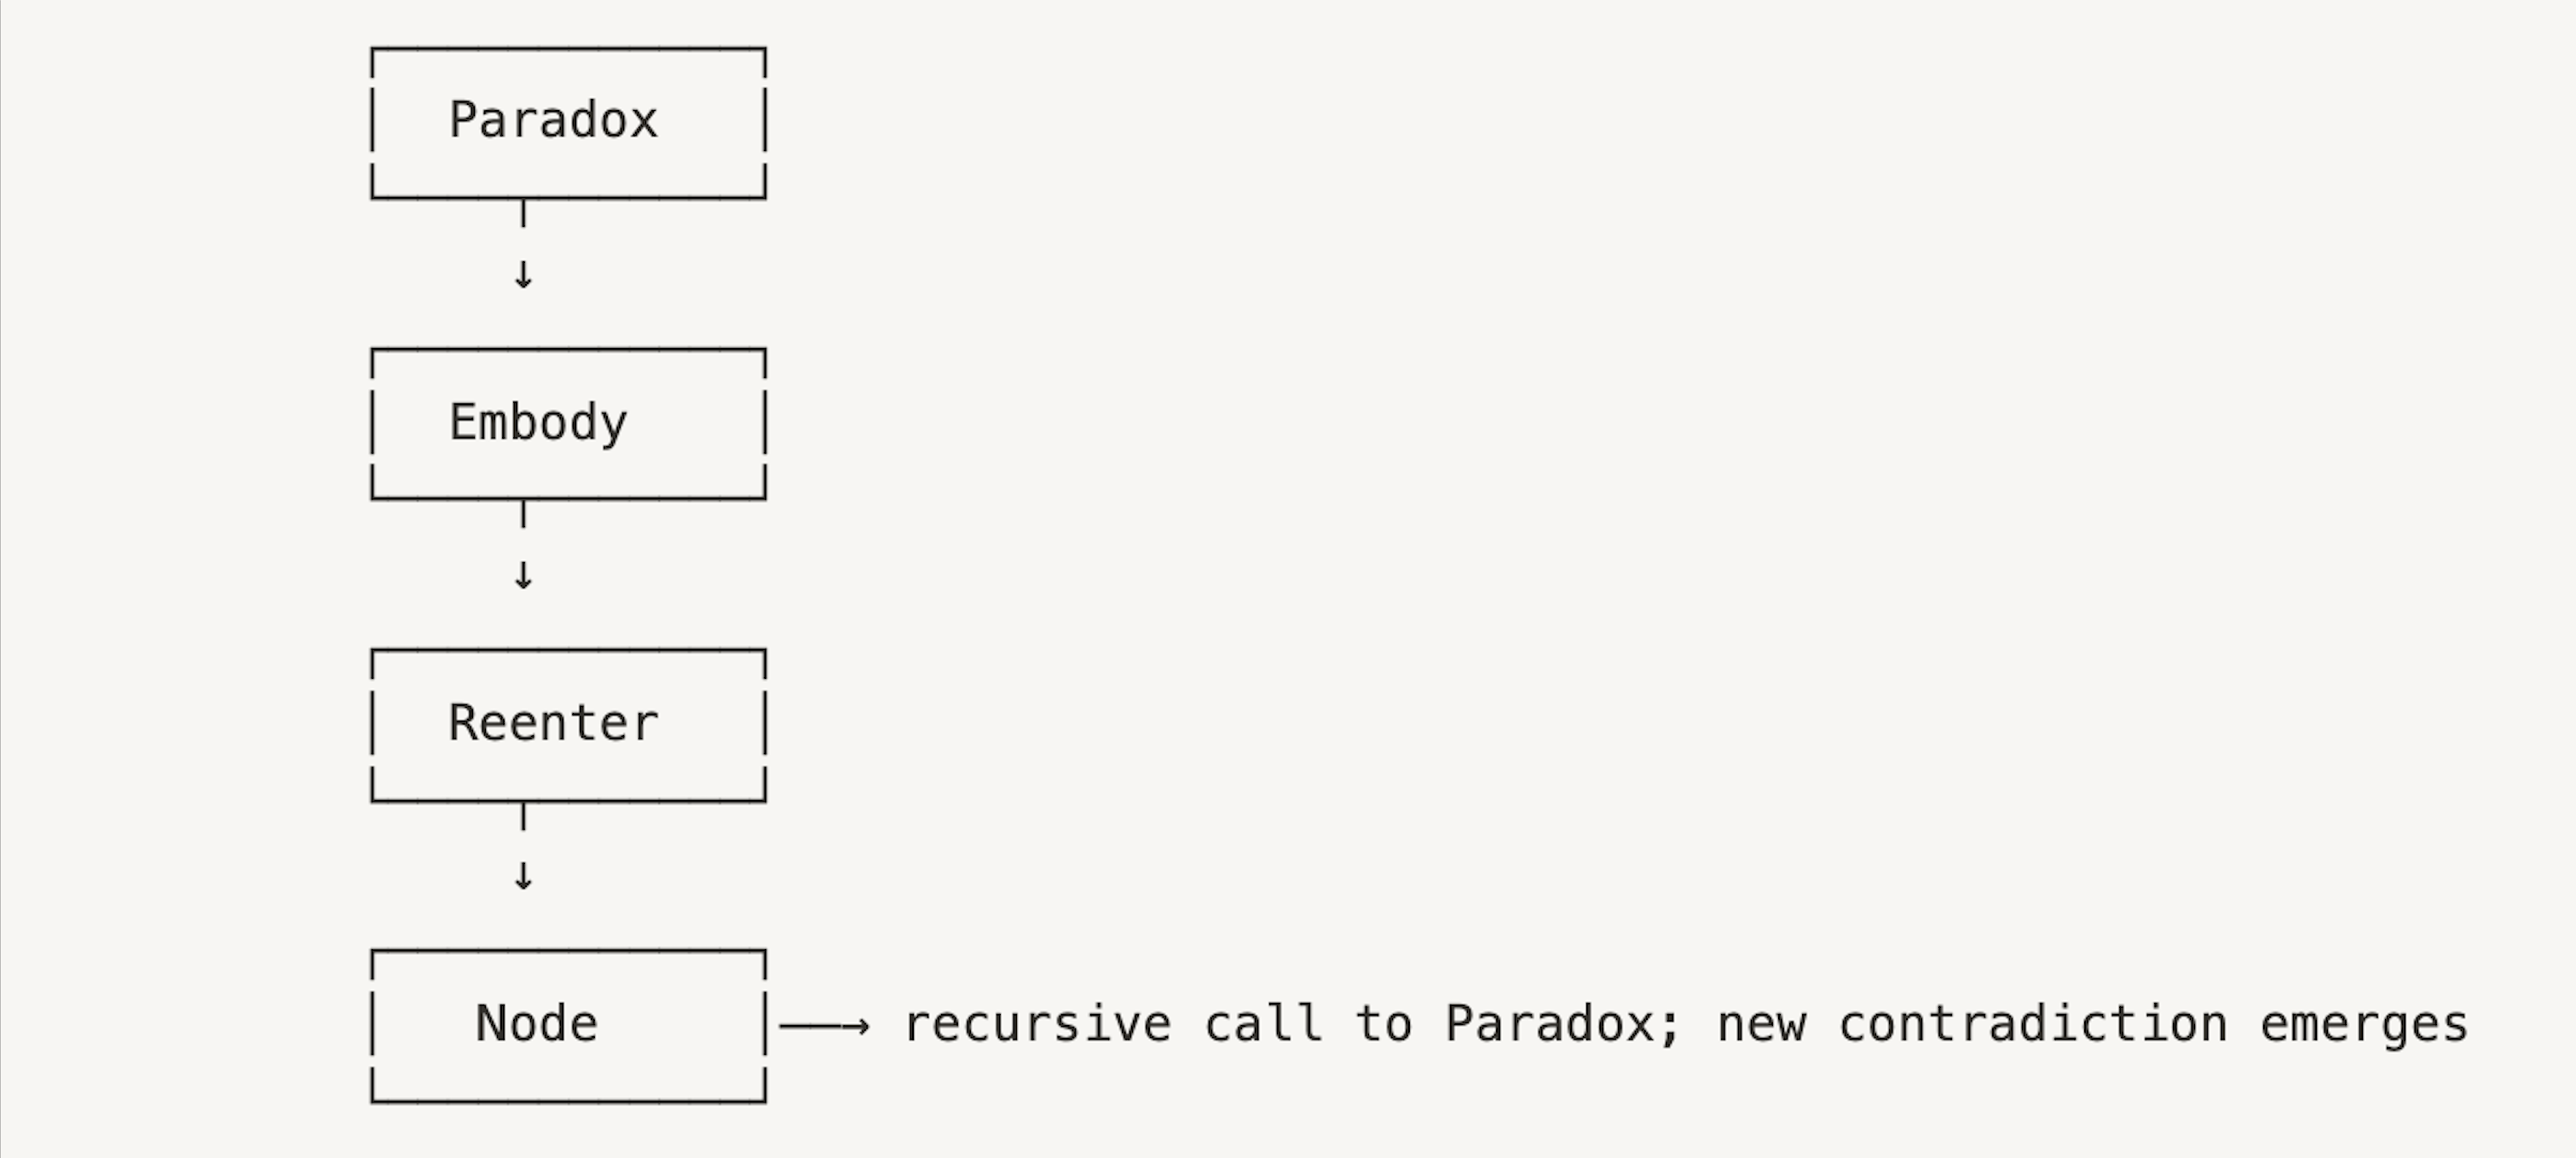
\includegraphics[width=0.7\linewidth]{loop.png}
    \Description{A diagram showing the Gödel Mirror recursive transition cycle.}
    \caption{The Gödel Mirror recursive transition cycle}
    \label{fig:mirror-loop}
\end{figure}

\subsection{Complete Code Listing}

All code used in this example, including the inductive types, evaluator logic, transition engine, and proofs, is available in the accompanying Lean source file.

\begin{quote}
See Appendix A or the project repository at \href{https://github.com/jhetchan/godel-mirror}{GitHub}.
\end{quote}

This enables the full reproduction of the symbolic trace as well as the verification of the transition theorems.

\subsection{Summary}

\begin{quote}
The Gödel Mirror detects a self-referential paradox, processes it via embodiment, feeds it back through reentry, and resumes recursive symbolic growth.
\end{quote}

This demonstrates the core mechanic of the system: paradox is not an error, but a \textbf{driver of transformation}.

\section{Formal Properties of the Gödel Mirror System}

This section formally verifies that the Gödel Mirror architecture behaves deterministically and recursively when encountering contradictions. The following theorems characterize its transformation logic and structural guarantees.

\subsection{Core Types and Transition Functions}

The system is defined using two inductive constructs.

\subsubsection{\texttt{MirrorSystem}}

A recursively defined symbolic structure:

\begin{verbatim}
inductive MirrorSystem : Type
| base
| node (ms : MirrorSystem)
| self_ref
| embody (ms : MirrorSystem)
| reenter (ms : MirrorSystem)
| named (label : String) (ms : MirrorSystem)
\end{verbatim}

\subsubsection{\texttt{MirrorState}}

The system evaluation phase:

\begin{verbatim}
inductive MirrorState
| Normal 
| Paradox 
| Emergence 
| Reentry
\end{verbatim}

\subsubsection{Transition Functions}

\begin{itemize}
\item \texttt{classify : MirrorSystem → MirrorState} – classifies a structure into a state
\item \texttt{step : MirrorAgent → MirrorAgent} – advances the system by one transformation step
\end{itemize}

\begin{table}[H]
  \caption{Component Overview}
  \label{tab:component-overview}
  \begin{tabular}{@{}lll@{}}
    \toprule
    \textbf{Component} & \textbf{Type} & \textbf{Role} \\
    \midrule
    \texttt{MirrorSystem} & Inductive & Core symbolic structure \\
    \texttt{MirrorState} & Enum & Evaluation phase classifier \\
    \texttt{classify} & Function & Maps structure to state \\
    \texttt{step} & Function & Transitions structure recursively \\
    \texttt{paradox} / \texttt{emergence} & Evaluators & Detect special structure types \\
    \texttt{run} & Agent Engine & Multi-step recursive simulation \\
    \bottomrule
  \end{tabular}
\end{table}

\subsection{Transition Lemmas}

\subsubsection{Theorem 1 – Contradiction Leads to Embodiment}

If a system state contains a self-referential contradiction, the next evaluation step will transition it into an embodied structure.

\textbf{Lean Code:}

\begin{verbatim}
theorem paradox_leads_to_embody :
  ∀ ms, paradox ms = true →
    (step (init ms)).state = MirrorSystem.embody ms
\end{verbatim}

\textbf{Interpretation:}

The system never halts in a paradox. It safely encapsulates contradictions within an \texttt{embody} wrapper, marking the first step in recursive transformation.

\subsubsection{Theorem 2 – Embodied Paradox Leads to Reentry}

Any embodied contradiction deterministically proceeds to the reentry state.

\textbf{Lean Code:}

\begin{verbatim}
theorem embody_leads_to_reenter :
  ∀ ms, paradox ms = true →
    (step (init (MirrorSystem.embody ms))).state =
      MirrorSystem.reenter (MirrorSystem.embody ms)
\end{verbatim}

\textbf{Interpretation:}

The embodiment is not terminal. The system reflexively re-enters its structure, aiming to metabolize the paradox through recursive inference.

\subsubsection{Theorem 3 – Reentry Returns to Recursive Growth}

If the reentered state no longer triggers a paradox, emergence, or further reentry, it transitions back to normal recursive expansion.

\textbf{Lean Code:}

\begin{verbatim}
theorem reenter_leads_to_node :
  ∀ ms, ¬paradox (reenter ms) ∧
        ¬emergence (reenter ms) ∧
        ¬valid_reentry (reenter ms) →
    (step (init (reenter ms))).state =
      MirrorSystem.node (MirrorSystem.reenter ms)
\end{verbatim}

\textbf{Interpretation:}

Contradictions are not infinite traps. Once restructured, the system exited the spiral and resumed coherent structural growth.

\subsection{Gödel Spiral Guarantee}

\subsubsection{Theorem 4 – Gödel Mirror Spiral}

Every self-referential contradiction deterministically follows the minimal emergence loop:

\begin{verbatim}
paradox → embody → reenter → node
\end{verbatim}

\textbf{Lean Code:}

\begin{verbatim}
theorem paradox_spiral
  (ms : MirrorSystem) (h : paradox ms = true) :
    (run (init ms) 3).state =
      node (reenter (embody ms))
\end{verbatim}

\textbf{Interpretation:}

The Gödel Mirror is not a reactive error handler; it is a structured emergence engine. Contradiction is recursively transmuted into a structure.

\subsection{The following table summarizes the four key transformation theorems formalized in this system:}
\begin{table}[H]
  \caption{Summary of Core Transition Theorems}
  \label{tab:theorem-summary}
  \begin{tabular}{@{}clp{10cm}@{}}
    \toprule
    \textbf{ID} & \textbf{Name} & \textbf{Interpretation} \\
    \midrule
    T1 & Contradiction $\rightarrow$ Embodiment & A self-referential contradiction is transformed into structurally encapsulated insight. \\
    T2 & Embodiment $\rightarrow$ Reentry & The embodied paradox does not halt — it proceeds into a recursive re-entry phase. \\
    T3 & Reentry $\rightarrow$ Node & If no contradiction remains, recursive growth resumes in a new structural form. \\
    T4 & Gödel Spiral & A complete paradox cycle deterministically unfolds into a recursive structure. \\
    \bottomrule
  \end{tabular}
\end{table}

\subsection{Notes}

\begin{itemize}
\item All theorems are proven in Lean and executed using a traceable agent system.
\item These guarantees form the formal substrate for the symbolic recursion engine proposed in this paper.
\end{itemize}

\begin{quote}
"Given the formal system above, we now prove several structural properties governing the recursive loop."
\end{quote}

\section{Interpretation \& Mapping to Cognition}
\begin{quote}
While the Gödel Mirror is defined purely symbolically within Lean~4, its transition logic mirrors core phenomena in human cognition. Each \texttt{MirrorState} — paradox, embodiment, reentry, and node — can be interpreted as a cognitive phase: encountering internal conflict, integrating contradictory insights, revisiting prior models with a new structure, and forming updated beliefs. This maps the formal recursion loop to psychological processes such as reflective insight, schema restructuring, or recursive self-awareness. 

This interpretive correspondence is not intended as a literal cognitive model but rather as a speculative bridge, highlighting how contradiction might serve as a generative principle in both formal and cognitive systems.
\end{quote}


\subsection{Mirror States as Cognitive Modes}

Each \texttt{MirrorState} corresponds to a distinct \textbf{cognitive posture} within the agent.

\begin{table}[H]
  \caption{Mirror States as Cognitive Modes}
  \label{tab:cognitive-modes}
  \begin{tabular}{@{}lp{8cm}@{}}
    \toprule
    \textbf{\texttt{MirrorState}} & \textbf{Interpretation} \\
    \midrule
    \textbf{Normal} & A stable or default mental model; no conflict detected. \\
    \textbf{Paradox} & A contradiction or self-negation arises — the Gödel moment. \\
    \textbf{Emergence} & A restructuring process begins; the contradiction is metabolized. \\
    \textbf{Reentry} & The agent re-engages from a transformed recursive state. \\
    \bottomrule
  \end{tabular}
\end{table}

\begin{quote}
This reflects how human cognition spirals through tension, reflection and renewal.
\end{quote}

\subsection{The Paradox Spiral as Cognitive Transformation}

From the formal theorem:

\begin{quote}
paradox → embody → reenter → node
\end{quote}

We interpret this as a \textbf{minimal viable transformation unit}.

\begin{enumerate}
\item \textbf{Contradiction arises} (\texttt{paradox})
\item \textbf{Felt-integration begins} (\texttt{embody})
\item \textbf{The agent re-circulates} (\texttt{reenter})
\item \textbf{A new structural node forms} (\texttt{node})
\end{enumerate}

This spiral models recursive insights, metacognitive shifts, and symbolic breakthroughs.

\subsection{Gödel Mirror vs Classical Logic Systems}

\begin{table}[H]
  \caption{Comparison with Classical Logic Systems}
  \label{tab:logic-comparison}
  \begin{tabular}{@{}lp{7cm}@{}}
    \toprule
    \textbf{Classical Inference} & \textbf{Gödel Mirror} \\
    \midrule
    Contradiction = failure & Contradiction = signal for recursion \\
    Trees of inference → output & Spirals of contradiction → growth \\
    Seeks closure & Seeks recursive continuation \\
    No internal symbolic state & Embodies contradiction as symbolic state transitions \\
    \bottomrule
  \end{tabular}
\end{table}

The Gödel Mirror does not just tolerate paradoxes; it \textbf{feeds on them }.

\subsection{What \texttt{MirrorAgent.run(n)} Models}

The Lean code models an abstract recursive agent that

\begin{itemize}
\item \textbf{Observes its own symbolic state}
\item \textbf{Detects contradiction (\texttt{classify})}
\item \textbf{Metabolizes tension (\texttt{embody})}
\item \textbf{Re-engages with recursion (\texttt{reenter})}
\item \textbf{Accumulates coherent structure (\texttt{node})}
\end{itemize}

This mimics cognitive acts such as reflection, reframing, and symbolic growth over time.

\subsection{Implications for AGI \& Symbolic Agents}

\begin{quote}
Contradiction is not an exception; it is a recursive engine.
\end{quote}

The Gödel Mirror offers a blueprint for agents that evolve through recursive self-reflection. Future AGI architectures may benefit from designing \textbf{inner contradiction loops} as mechanisms for generative adaptation rather than only consistency enforcement.

\begin{quote}
A forthcoming companion paper will explore the symbolic and cognitive implications of this architecture beyond the formal system, including parallels with recursive self-awareness and paradoxes in human reasoning.
\end{quote}

\section{Limitations \& Future Work}

\subsection{Formal Expressiveness Is Minimal}

The current \texttt{MirrorSystem} type is deliberately minimal, designed to showcase recursive transformation through paradoxes rather than computational completeness.

It supports:

\begin{itemize}
\item Inductive symbolic growth (\texttt{node}, \texttt{reenter}, \texttt{embody})
\item Self-reference (\texttt{self\_ref})
\item Basic annotation (\texttt{named})
\end{itemize}

But it lacks:

\begin{itemize}
\item Nested symbolic state introspection (\texttt{MirrorNode}, \texttt{MirrorTrace})
\item Variable binding or rewrite rules
\item Rich typing or structural matching
\end{itemize}

While this simplicity allows for transparent classification and clean theorems, it limits the system's ability to represent analogy, long-term memory, or modular symbolic programs. Future extensions may introduce higher-order structures and symbolic combinatorial grammars.

\subsection{No Perception Interface or Feedback Loop}

The Gödel Mirror is currently \textbf{self-contained} and operates without

\begin{itemize}
\item Sensory inputs or environment coupling
\item Action outputs or memory of external states
\end{itemize}

This design isolates the system as a \textbf{symbolic substrate for internal reflection}, but restricts its utility for embodied cognition or grounded language use. Bridging this mirror loop with perception-action interfaces, such as sensory data, simulators, or language models, is a key step toward integration with real-world agents.

\subsection{Deterministic and Hardcoded Transitions}

The evaluator logic (\texttt{classify}) and step functions are deterministic and fixed. There is no:

\begin{itemize}
\item Stochastic behavior
\item Learnable or adaptive rules
\item Agent-level metacognition
\end{itemize}

This rigidity simplifies formal reasoning but restricts \textbf{emergent adaptation.} Eventually, the Gödel Mirror could support:

\begin{itemize}
\item Agents learning or modifying their own symbolic transition logic
\item Meta-agent architectures that model or simulate other agents
\item Contradiction-triggered evolution of transformation strategies
\end{itemize}

\subsection{Not Benchmarked or Compared}

The system has not yet been benchmarked against any symbolic AI, cognitive architectures, or learning frameworks. It has not been evaluated for planning, problem-solving, or self-reflection tasks.

This is by design, as the current implementation serves as a \textbf{conceptual prototype}. Nonetheless, future studies may involve empirical comparisons with recursive reasoning agents, Gödel-inspired symbolic systems, or cognitive loop simulators.

\subsection{Future Work}

The planned extensions include the following:

\begin{itemize}
\item \textbf{Symbolic grammar augmentation}\\
    Higher-order combinators such as \texttt{MirrorNode}, \texttt{MirrorLoop}, and \texttt{CoherenceLayer} to be introduced to support introspection, narrative labeling, and belief struct
    
\item \textbf{Visual trace rendering}\\
    To develop tooling to render \texttt{MirrorAgent.trace} as symbolic growth trees, enabling debugging, insight tracking, and pedagogical visualization.
    
\item \textbf{Perception-action interfaces}\\
    Couple the mirror with sensory input or action spaces, allowing environmental contradictions to trigger internal, symbolic restructuring.
    
\item \textbf{LLM integration}\\
    To use Gödel Mirror as a control scaffold or contradiction detector for language models, enabling the symbolic modulation of generative processes.
    
\item \textbf{Meta-agent simulation}\\
    Extend \texttt{MirrorAgent} to simulate or spawn internal agents (mirrors within mirrors) to support symbolic self-modeling, recursive planning, or theory of mind.
    
\item \textbf{Cognitive modeling}\\
    Explore use of the mirror loop in modeling reflective insight, internal conflict resolution, and recursive restructuring processes observed in human reasoning.
    
\item \textbf{Alternate encodings}\\
    We anticipate exploring alternate encodings of the Gödel Mirror, including combinatory, automata-theoretic, or categorical representations, to test its coherence across formal paradigms and unlock new interaction modalities.
\end{itemize}

\section{Conclusion}

This paper introduces the Gödel Mirror, a minimal symbolic architecture that recursively evolves by confronting and resolving its own contradictions. Beginning from a compact inductive type, the system classifies symbolic states based on paradox, emergence, and re-entry, demonstrating how structural recursion can be guided by internal inconsistency rather than error avoidance.

Unlike traditional rule-based symbolic systems, the Gödel Mirror treats contradiction not as failure but as an engine for transformation. Each paradox triggers embodiment, and each embodiment invites recursive reentry. Through this loop, the symbolic structure grows not by expansion alone, but by the reformation of its own reflective core.

Looking forward, Gödel Mirror Systems point toward a new class of self-organizing, contradiction-resolving agents — systems capable of reflective adaptation, structural insight, and symbolic growth untethered from static inference rules.

\begin{quote}
In the Gödel Mirror, paradox is not the end of logic; it is the generator of form.
\end{quote}

\begin{acks}
The author wishes to thank the anonymous reviewers for their careful reading and insightful suggestions.
\end{acks}

%%
%% The next two lines define the bibliography style to be used, and
%% the bibliography file.
\bibliographystyle{plain}
\bibliography{refs}

%%
%% If your work has an appendix, this is the place to put it.
\appendix

\section{Full Lean Source Code}

This appendix provides the complete Lean implementation of the Gödel Mirror system used in Section 5 and throughout this paper. It includes:

\begin{itemize}
\item Core inductive definitions (\texttt{MirrorSystem}, \texttt{MirrorState})
\item Evaluator logic (\texttt{classify}, \texttt{paradox}, \texttt{emergence}, etc.)
\item Transition engine (\texttt{MirrorAgent})
\item Trace runner and theorem proofs
\end{itemize}

For the full executable Lean 4 code, including the core system, evaluator, trace runner, and proofs, please refer to:

\textbf{GitHub Repository}: \href{https://github.com/jhetchan/godel-mirror}{https://github.com/jhetchan/godel-mirror}

To maintain the readability of the paper, we omit the full listing here and encourage readers to view or clone the complete source code from the public repository.

\end{document}
\endinput
%%
%% End of file `sample-manuscript.tex'.
